\section{Graph neural networks}
\label{sec:ch10:gnns}

Throughout this book, we have focused on ways in which you can represent and, if desired *conceptualize*, network-valued data that place it in a context in which you can apply many of the algorithms you are used to. 

For instance, in the case of the spectral embedding in {numref}`ch6:spectral`, we devised techniques which allow you to take a network of nodes and edges, and construct a tabular array with which you can learn about using traditional techniques like $k$-means for community detection in {numref}`ch7:comm_detect`, or other tasks of interest you might have. We learned how this representation had underpinnings in the rdpg from {numref}`ch5:rdpg`, and how you could use this as a conceptual basis to assign explicit assumptions you might make about your network in order for you to do downstream statistical inference, such as if you want to compare two networks in {numref}`ch8:twosample`. 

In this section and the next on diffusion methods in {numref}`ch10:diffusion`, we are going to turn this approach somewhat on its head, and investigate approaches which, at face value, appear to fundamentally alter existing techniques which you already might know about, neural networks, to make them amenable to network-valued data directly.

## The drug discovery problem

In chemistry, a *molecule* is a group of atoms which are bonded together. If you haven't taken a chemistry course, you can think of an atom as a *building block*, and a *bond* as the *glue* that holds the molecule together. Every interaction you have with the world occurs through molecules; the water you drink, for instance, is a molecule consisting of hydrogen and oxygen, $H_20$, and the air you breathe consists most of molecules of nitrogen $N_2$, small amounts of oxygen $O_2$, and trace amounts of argon $Ar$ and carbon dioxide $CO_2$. In these formulas, the letters represent a particular atom, and the subscripts represent the number of these atoms in the molecule.

Without getting too deep into the chemistry, a fundamental problem for many pharmaceutical and chemistry investigations involves the analysis of molecules that might be useful for clinical purposes. A *clinically useful molecule* is a molecule which has properties which, for one reason or another, might make it beneficial for humans. For instance, if you. have ever had a headache, you have probably become familiar with a molecule $C_{13}H_{18}O_2$, or Ibuprofen (Advil).

Many of the drugs that we are familiar with on an everyday basis have, it turns out, been discovered totally by accident. For a laugh, we'd encourage you to check out the discovery of penicillin from {cite:p}`ContributorstoWikimediaprojects2023Jan`, which is a family of molecules having a core structure of $C_9H_{11}N_2O_4S$. 

Unfortunately, coming across all of these "happy accident" molecules has become more and more infrequent as pharmaceuticals have progressed. When a given condition is identified that a pharmacologist decides to attempt to devise a treatment for, they often must proceed facing several enormous hurdles for candidate molecules. The molecules must be:
1. non-toxic to humans,
2. an appropriate size,
3. be readily absorbed by humans, and
4. able to address the condition of interest.

Achieving all of these aims is extremely difficult, and extremely risky in terms of time, labor, and most of all potential risk to human participants in drug trials. Determining definitive, or at least suggestive, evidence that the molecule will achieve any or all of these conditions *before* running live human tests can save the company billions of dollars and can save participants in drug trials unnecessary exposure to harm.

Running laboratory tests to screen these molecules is an expensive, time-consuming, and skilled labor-intensive process: what are the companies left to do?

Many drug companies utilize virtual screening methods in which computational methods are used to quickly search large libraries of molecules to filter ones with the desirable properties. Success in virtual screening methods are determined by the accuracy and speed of the computational approach. For instance, molecular dynamics simulates the physical movement of each atom and particle, thus providing the most accurate calculations of molecular properties, but requires an intractable number of numerical calculations that makes it infeasible to use in practice. Instead, methods have been built around succint 2D representations of molecules, further compressed in 1D SMILES {cite:p}`Weininger1988Feb` {cite:p}`Weininger1989May` {cite:p}`Weininger1990Aug` strings (Simplified molecular-input line-entry system), that summarize the structural relationships between different atoms through the chemical bonds connecting them. These $1D$ strings are known as *fingerprints* for the molecules, and are illustrated in Figure \ref{fig:next:smiles}.

\begin{figure}
    \centering
    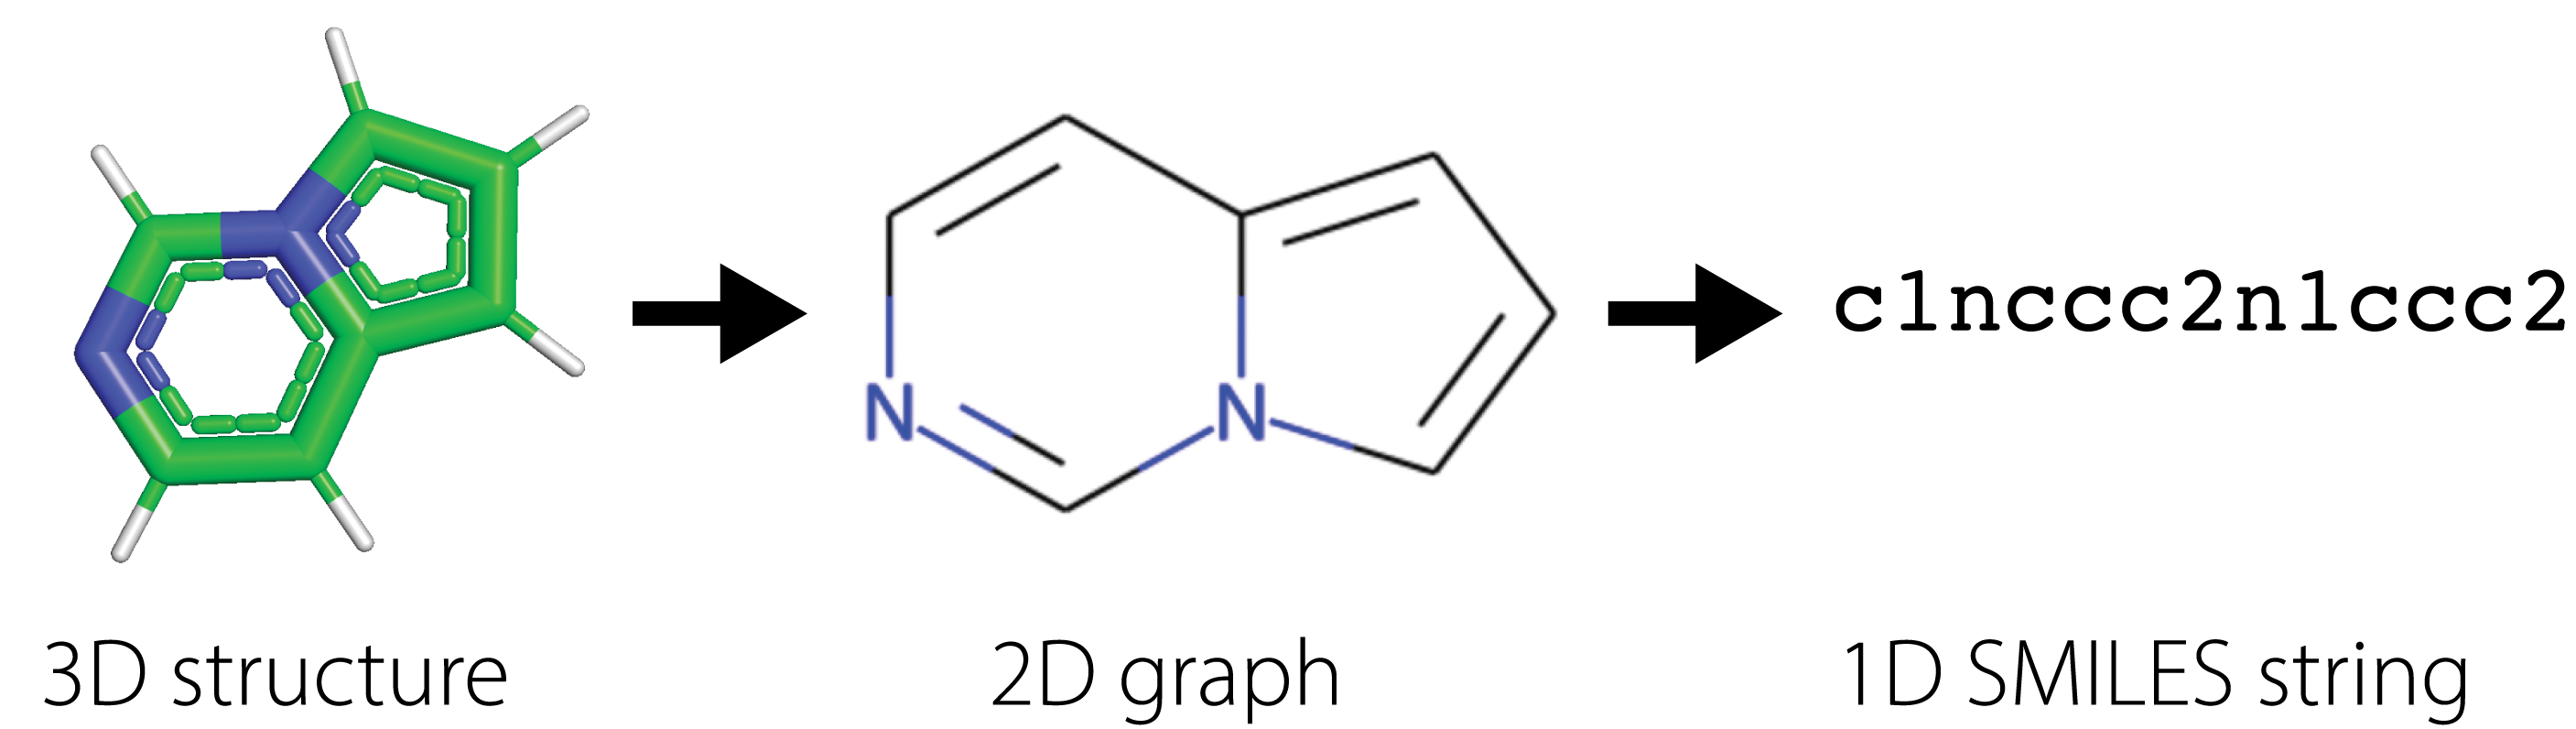
\includegraphics[width=\linewidth]{next/Images/molecule_repr.png}
    \caption[SMILES string for a molecule]{A SMILES string for a molecule.}
    \label{fig:next:smiles}
\end{figure}

Using SMILES, practioners have built statistical models to estimate correlations between SMILES and different molecular properties. These traditional methods have relied on building hand-crafted features derived from SMILES and optimizing simplistic statistical models to predict molecular properties from fingerprints of the molecules. 

This too, however, is extremely labor intensive and, most importantly, requires direct human intervention to decipher the features used for statistical learning. With some clever manipulation, scientists have identified an ingenius approach to turn molecular screening into a network learning problem.

### Obtaining a network from a molecule

In our initial description of a molecule, we described that a molecule was just a group of atoms which are bonded together. How can we conceptualize this as a network?

If we think of the atoms of the molecule as the nodes of the network, and the bonds as the edges, this problem is extremely straightforward. Let's see how this would work with a single molecule of water. Remember that water has the molecular formula $H_2O$, which means that it is two hydrogen atoms, and one oxygen atom. The molecular structure of water is that the oxygen atom basically sits in the middle, and the hydrogens hang off the side. The process of turning a molecule into a network is illustrated in Figure \ref{fig:next:molecule}. In \textbf{(A)}, the structure of a molecule is illustrated, which is identified through experimentation by chemists. \textbf{(B)} shows the process of turning a molecule into a network, where the atoms (oxygen and two hydrogens) become the nodes of the network, and the bonds between the oxygen atom and the hydrogens become the edges. \textbf{(C)} illustrates the network as an adjacency matrix.

\begin{figure}
    \centering
    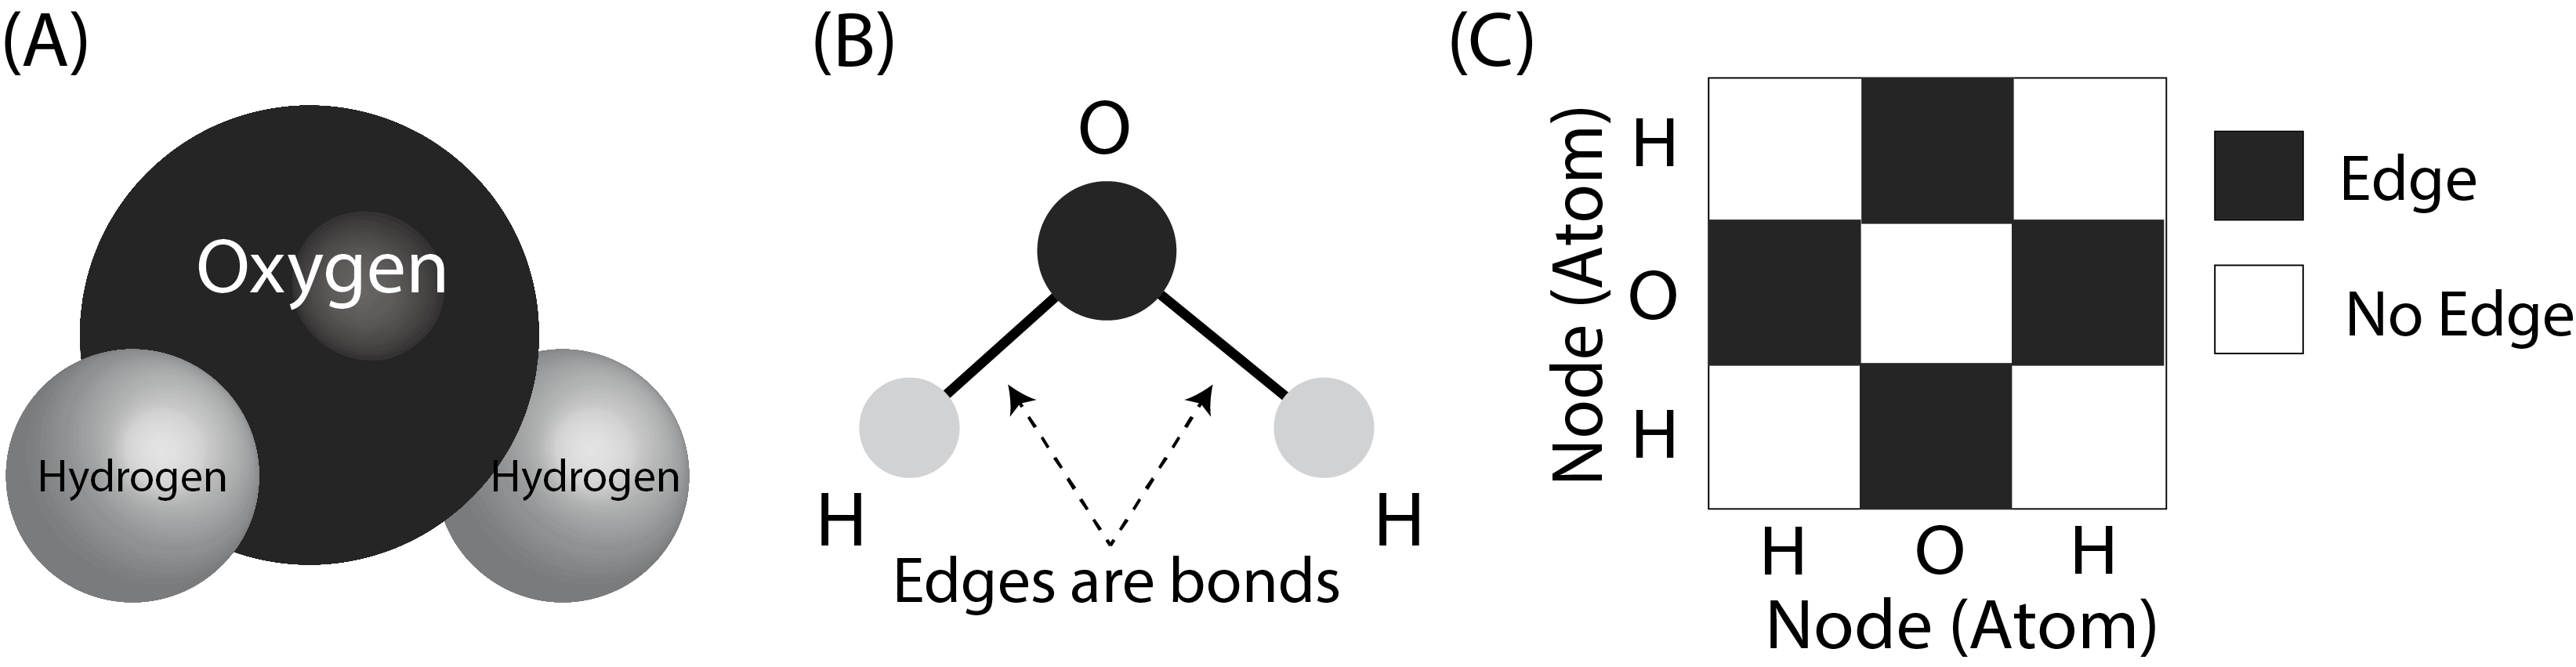
\includegraphics[width=\linewidth]{next/Images/water_molecule.png}
    \caption{\textbf{(A)} a molecular structure for water ($H_2 O$), \textbf{(B)} a network representation of a water molecule, \textbf{(C)} the network as an adjacency matrix.}
    \label{fig:next:molecule}
\end{figure}

Given a fingerprint (the SMILES string), this molecular structure, and consequently the network and the adjacency matrix, are fully determined. The inverse is also true: given a network and the other attributes of the atomic structure, the fingerprint can be determined. Implicitly, computational strategies which produce desirable representations of the fingerprints produce a desirable representation for the network itself.


### Our network learning problem

For this section, we will focus our attention on the first hurdle faced by pharmacoligists. Provided a SMILES fingerprint for a molecule, we would like to determine whether the molecule is toxic or non-toxic.

## Preprocessing SMILES fingerprints

We will be using one of the datasets packaged in \texttt{MoleculeNet} \cite{moleculenet}. PyTorch Geometric (PyG) \cite{pytorchgeom,pytorch} provides a convenient module to access it. We first import the module `MoleculeNet` then extract the `ClinTox` dataset \cite{Novick2013Nov}. The dataset has a total of $1478$ molecules labeled with their presence or absence of toxicity -- determined from clinical trials done by the Food & Drug association (FDA). Since this is a binary classification task, we observe there are two classes.

\begin{lstlisting}[style=python]
from torch_geometric.datasets import MoleculeNet

dataset = MoleculeNet(root='data/clintox', name='ClinTox')
print(f'Dataset: {dataset}\nNumber of molecules/graphs: {len(dataset)}\nNumber of classes: {dataset.num_classes}')
\end{lstlisting}

Let's look at a few molecules to understand their networkstructure. Each molecule has a known 3D structure and an associated SMILES string. We pick out two arbitrary molecules from the dataset, and take a look first at their SMILES string:

\begin{lstlisting}[style=python]
mols = dataset[26], dataset[83]
[print(m.smiles) for m in mols];
\end{lstlisting}

Next, we can draw the molecular structures for the two molecules:

\begin{lstlisting}[style=python]
from rdkit import Chem
from rdkit.Chem.Draw import rdMolDraw2D
from IPython.display import SVG

smiles = [Chem.MolFromSmiles(m.smiles) for m in mols]
d2d = rdMolDraw2D.MolDraw2DSVG(600,280,300,280)
d2d.drawOptions().addAtomIndices = True
d2d.DrawMolecules(smiles)
d2d.FinishDrawing()
SVG(d2d.GetDrawingText())
\end{lstlisting}

The networks each have a different number of nodes (atoms). Further, each node has a number which uniquely identifies that node in the molecule. These molecules have been analyzed with cheminformatics software, \texttt{RDKit} \cite{rdkit}, and also come with a set of node attributes for descriptive characteristics of that node in the particular molecule. While these node attributes are not relevant for our tutorial, they have substantial real-world applications to optimize predictive accuracy. Let's take a look at the number of atoms and the number of atomic features now:

\begin{lstlisting}[style=python]
for i,m in enumerate(mols):
    print(f'Molecule {i+1}: Number of atoms={m.x.shape[0]}, Features per atom={m.x.shape[1]}')
\end{lstlisting}

As we discussed above, the edges of the network are the bonds between different pairs of atoms (the nodes). Using the SMILE fingerprint, we can also obtain information of the bonds of the network. Let's take a look at the indices of the bonds, shown below:

\begin{lstlisting}[style=python]
d2d = rdMolDraw2D.MolDraw2DSVG(600,280,300,280)
d2d.drawOptions().addBondIndices = True
d2d.DrawMolecules(smiles)
d2d.FinishDrawing()
SVG(d2d.GetDrawingText())
\end{lstlisting}

Unlike many of the networks we have seen in examples so far, the adjacency matrices for molecular networks tend to be, especially for larger molecules (molecules with more nodes, or atoms) extremely sparse, a concept that we covered in Section \ref{sec:ch7:sparse}. In smaller networks, this is a rather irrelevant consideration. Remember that the adjacency matrix has, for a simple network, $\binom n 2 = \frac{1}{2}n(n - 1)$ possible edges. So, if we store the entire adjacency matrix, we need to keep track of $\frac{1}{2}n (n - 1)$ entries. 

In a sparse adjacency matrix, the total number of edges might be considerably less than this. Remember that an edge is indexed by two nodes, so if two times the number of edges is less than $\binom n 2$, we can save a lot of space by storing and operating on the adjacency matrix using edgelists.

When you have a network with a sparse adjacency matrix, you can even perform many matrix computations without ever having to construct the (potentially large) adjacency matrix in its entirety. In Section \ref{sec:ch7:sparse}, we discussed the implications directly using \texttt{scipy} for sparse matrices. An equivalent construct for graph neural networks are \texttt{pytorch} sparse arrays such as those we leverage here, which similarly operate a lot faster and more efficiently on adjacency matrices which are sparse.

With this in mind, when we look through the dataset, we need to keep in mind that the network is stored using this sparse edgelist format. To build the adjacency matrix so that we can visualize it using the traditional heatmap, we need to first construct the adjacency matrix from the edgelist, which is what we do below:

\begin{lstlisting}[style=python]
import numpy as np

_process = lambda x: [e[0] for e in np.split(x, 2)]
def A_from_edgelist(molecule):
    """
    A function that takes molecules, and produces an adjacency matrix.
    """
    # the number of nodes is the number of atoms (rows of .x attribute)
    n = molecule.x.shape[0]
    # the adjacency matrix is n x n
    A = np.zeros((n, n))
    edgelist = m.edge_index.numpy()
    # loop over the edges e_k, and for each edge, unpack the 
    # nodes that are incident it. for this corresponding pair of nodes, 
    # change the adjacency matrix entry to 1
    for e_k, (i, j) in enumerate(zip(*_process(edgelist))):
        A[i, j] = 1
    return A
\end{lstlisting}

Now that we can produce adjacency matrices from sparse edgelists, we can convert the molecules to adjacency matrices, and then plot them using heatmaps like we are used to:

\begin{lstlisting}[style=python]

\end{lstlisting}



\begin{lstlisting}[style=python]

\end{lstlisting}



\begin{lstlisting}[style=python]

\end{lstlisting}



\begin{lstlisting}[style=python]

\end{lstlisting}



\begin{lstlisting}[style=python]

\end{lstlisting}



\begin{lstlisting}[style=python]

\end{lstlisting}



\begin{lstlisting}[style=python]

\end{lstlisting}


